\chapter{}
\section{电负性,偶极矩,杂化效应}
\label{sec:2.1}

\subsection{电负性}
\label{sec:2.1.1}
$\underset{(\chi)}{\text{电负性}}\uuline{\mathrm{def}}\text{原子对}\underset{\text{成键电子}}{\underline{\text{键合电子}}}\text{的吸引}
\underset{\text{抢$e^-$能力}}{\uwave{\text{能力}}}$大小

(1)横向$\quad\text{核电荷}\uparrow\quad\text{吸引力}\uparrow\quad\chi\uparrow$

\qquad $\Rightarrow\chi_{F}>\chi_{O}>\chi_{N}>\chi_{C}$

(2)纵向:外层$e^-$数(不变)$\quad\text{层数}\uparrow\quad\text{吸引}\uparrow\quad\chi\uparrow$

\qquad $\Rightarrow\chi_{F}>\chi_{Cl}>\chi_{Br}>\chi_{I}$

\subsection{极性键与部分电荷$\delta+/-$}
\label{sec:2.1.2}

$A-B\qquad\underset{\text{相差大}}{\chi_{A}\neq\chi_{B}}\rightarrow\text{电子云偏移}\rightarrow\text{A-B为极性键}$

若A与B的$\chi\text{值相差不大,则为非极性键}\quad\text{无}\delta^+/\delta^-$

\subsection{杂化效应}
\label{sec:2.1.3}
杂化效应\quad $(\text{比较}\underset{sp}{\ce{-C#CH}},\underset{sp}{\ce{-CH=CH2}},\underset{sp}{\ce{-CH2CH3}}$的电负性)

从$sp\rightarrow sp^2 \rightarrow sp^3\quad\overset{sp^i}{\text{杂化指数i}}\uparrow\rightarrow\text{p轨道成分}\uparrow\rightarrow\text{电子云靠程度}\downarrow\rightarrow\text{电负性}\downarrow$

\qquad\qquad $\Rightarrow\underset{sp}{\chi_{\ce{-C#CH}}}>\underset{sp^2}{\chi_{\ce{-C=CH2}}}>\underset{sp^3}{\chi_{\ce{-CH2CH3}}}$

杂化效应:某相同原子的电负性会被杂化形态影响

\subsection{偶极,偶极矩}
\label{sec:2.1.4}
\begin{figure}[H]
    \begin{tikzpicture}[scale=.4]
        \draw[->] (0,0)--(2,0)node[black,pos=0,left]{偶极矩$\quad$记};
        \draw[-] (.3,.25)--(.3,-.25);
        \node[black] at (.3,-.5) {$\delta^+$};
        \node[black] at (2,-.5) {$\delta^-$};
    \end{tikzpicture}
\end{figure}

B-A为极性键,其中A带$\delta^{\oplus}\text{,B带}\delta^{\ominus}$

$\quad\text{定义矢量}\vec{\mu}\text{由}\delta^{\oplus}\rightarrow\delta^{\ominus}
\quad\text{大小}\left| \vec{\mu} \right|=q\left| \vec{\gamma} \right|\text{即}\vec{\mu}=q\vec{\gamma}\rightarrow
\begin{cases}
    \left| \vec{\mu} \right|_{\text{键}}=0\quad\text{非极性键} \\
    \left| \vec{\mu} \right|_{\text{键}}\neq 0\quad\text{极性键}
\end{cases}$

\qquad\qquad\qquad \text{称$\vec{\mu}$为A-B的键偶极矩}

分子偶极矩:若分子各键偶极矩矢量记为$\vec{\mu_1},\vec{\mu_2},\vec{\mu_3},\dots,\vec{\mu_n}$

\begin{equation}
    \text{记分子偶极矩}
    \underset{\text{矢量合成}}{\vec{\mu}=\sum_{i=1}^{n} \vec{\mu_i}}
\end{equation}

\begin{figure}[H]
    \centering
    \begin{subcaptionbox}
        \begin{tikzpicture}[scale=.5]
            \node[black,above] at (-.5,2) {eg.};
            \chemfig{C(-[:45,1.3]Cl)(=[:180,1.3]C(-[:135,1.3]H)(-[:-135,1.3]Cl))(-[:-45,1.3]H)};
            \node[black,above] at (7,0) {$\vec{\mu}=\vec{\mu_1}+\vec{\mu_2}=\vec{0}$};
            \node[black,below] at (7,0) {$\therefore$非极性分子};
            \draw[->] (2.5,.5)--(3.7,1.7)node[black,pos=.5,left] {$\vec{\mu_1}$};
            \draw[-] (2.5,.8)--(2.8,.5);
            \draw[->] (1.7,0)--(.5,-1.2)node[black,pos=.5,right] {$\vec{\mu_2}$};
            \draw[-] (1.7,-.3)--(1.4,0);
            \node[black] at (2,-1.5) {反式};
        \end{tikzpicture}
    \end{subcaptionbox}
    \begin{subcaptionbox}
        \begin{tikzpicture}[scale=.5]
            \chemfig{C(-[:45,1.3]Cl)(=[:180,1.3]C(-[:135,1.3]Cl)(-[:-135,1.3]H))(-[:-45,1.3]H)};
            \node[black,above] at (7.5,0) {$\vec{\mu'}=\vec{\mu_1'}+\vec{\mu_2'}\neq0$};
            \node[black,below] at (7.5,0) {$\therefore$极性分子};
            \draw[->] (3.3,0)--(4.5,1.1)node[black,pos=.5,right] {$\vec{\mu_1}$};
            \draw[-] (3.3,.3)--(3.6,0);
            \draw[->] (.9,0)--(-.3,1.1)node[black,pos=.5,left] {$\vec{\mu_2}$};
            \draw[-] (.9,.3)--(.6,0);
            \node[black] at (2,-1.5) {顺式};
            \draw[->] (2,.5)--(2,2)node[black,pos=.5,right] {$\vec{\mu'}$}node[black,above] {$\left| \vec{\mu}_{\text{分子}} \right|$};
            \draw[-] (1.8,.7)--(2.2,.7);
        \end{tikzpicture}
    \end{subcaptionbox}
\end{figure}

\section{有机反应的本质}
\label{sec:2.2}

\subsection{分子间作用阻碍三种形式}
\label{sec:2.2.1}
阻碍=$\underset{\text{(大)}}{\text{外层电子的库伦斥力}}+
\overset{\text{取向+诱导+色散}}{\overset{\Uparrow}{\underset{\text{(小)}}{\text{分子间作用力}}}}+\underset{\text{(大)}}{\text{轨道作用}}$

\quad $\downarrow$

克服阻碍的最小能$E_{min}\quad (\text{活化能}E_A)$

\quad $\downarrow\quad \text{分子间有效碰撞}\Rightarrow\text{克服阻碍}\Rightarrow$反应发生

$\underset{\text{(反应)}}{\text{克服阻碍}}=\underset{(1)}{\text{“净”电荷吸引}}+\underset{(2)}{\text{轨道作用}}$

\subsection{两种途径使反应发生}
\label{sec:2.2.2}

$\newline$
(1)$\underset{\textcolor{red}{\text{分子的作用}})}{\underset{(\textcolor{red}{\text{解释不了非极性}}}{\text{电荷吸引}}}
\begin{cases}
    \text{无机:纯离子反应}\quad eg.\ce{Ag^+ + Cl^- -> AgCl v}\quad  Ag^{\oplus}\overset{\text{吸引}}{\rightarrow\leftarrow}Cl^{\ominus} \\
    \underset{\text{(中性分子)}}{\text{有机:}}
    \begin{cases}
        \underset{\text{(偶极)}}{\text{离子与极性分子之间的作用}}\quad eg.^{\ominus}CN\overset{\text{吸引}}{\rightarrow\leftarrow}
        \overset{\delta^{\oplus}}{\chemfig{(=[:0]O)(-[:135]H)(-[:-135]H)}} \\
        \underset{\text{(偶极)}}{\text{极性分子间的作用}}\quad eg.\overset{\delta^{\ominus}}{\chemfig{\charge{0=\:}{O}(-[:135]H)(-[:-135]H)}}
        \overset{\text{吸引}}{\rightarrow\leftarrow}\overset{\delta^{\oplus}}{\chemfig{(=[:0]O)(-[:135]H)(-[:-135]H)}}
    \end{cases}
\end{cases}$

$\newline$
(2)轨道重叠\quad orbsoverlap\quad 对有机反应的解释

(反应1)Rxn1\quad 离子与极性分子的作用\quad $^{\ominus}CN+HCHO$
\begin{figure}[H]
    \begin{tikzpicture}[baseline=(current bounding box.center),scale=.5]
        \draw[->] (0,0)--(0,4)node[right] {Eorbs};
        \draw[draw=black] (-2,2)ellipse (.6 and .3);
        \fill (-1.6,2.1) circle (1pt);
        \fill (-1.6,1.9) circle (1pt);
        \node[right] at (-1.5,2) {$^{\ominus}CN$};
        \node[below] at (-1.5,1.7) {sp孤对电子};
        \draw (1,3)--node{$\uparrow\downarrow$}+(1,0)node[below]{$sp_c$};
        \draw[-] (8,3.5)--(9,3.5)node[right] {$\pi^{\oplus}_{co}$};
        \draw[->] (11,0)--(11,4)node[right] {Eorbs};
        \draw[->] (2.5,3)--(7.5,3.5)node[below,pos=.6] {轨道重叠使反应发生};
        \node[above] at (5.5,1) {形成$\pi\text{键的2个2p轨道的}e^-$};
        \node[below] at (5.5,1) {重新组合生成$\pi_{c-o}\text{与}\pi^*_{c-o}$两个};
        \node[below] at (3,0) {分子轨道};
    \end{tikzpicture}
    \chemfig{(=[:90]O)(-[:-30]H)(-[:-150]H)}
\end{figure}

\begin{figure}[H]
    \centering
    \begin{tikzpicture}[scale=.5]
        \draw[->] (-5.5,-2)--(-5.5,4)node[right]{Eorb(C=O)};
        \draw (-3.6,-.75)--node{$\uparrow\downarrow$}+(1,0)node[left,pos=0]{2s};
        \draw (-4.6,2.25)--++(.5,0)node{$\uparrow$}-- ++(.5,0)node[left,pos=0]{$2p$};
        \draw (-3.4,2.25)--++(.5,0)node{$\uparrow$}-- ++(.5,0)node[above,pos=0]{$C(2s^22p^2)$};
        \draw[decorate,decoration={brace, amplitude=2}, line width=.8] (-1.7,2.5)--(-1.7,-2);
        \draw (-1.4,.25)--++(.5,0)node{$\uparrow$}-- ++(.5,0)node[below]{$2\times sp^2$};
        \draw (-.2,.25)--++(.5,0)node{$\uparrow$}-- ++(.5,0);
        \draw[->] (-.4,-.75)--(-3,-2.75)node[below]{这两个$sp^2$与H成键};
        \draw (1,.25)--++(.5,0)node{$\uparrow$}-- ++(.5,0)node[below]{$sp^2$};
        \draw[->] (1.5,-.75)--(.5,-2)node[below]{这个$sp^2$形成C-O键};
        \draw[-,dashed] (2,.25)--(4,5);
        \draw[-,dashed] (2,.25)--(4,-1.5);
        \draw (1,2.75)--++(.5,0)node{$\uparrow$}-- ++(.5,0)node[left,pos=0]{$2p$};
        \draw[-,dashed] (2,2.75)--(4,4);
        \draw[-,dashed] (2,2.75)--(4,1);
        \draw (4,-1.5)--node{$\uparrow\downarrow$}+(1,0)node[right]{$\sigma_{c-o}$};
        \draw (4,1)--node{$\uparrow\downarrow$}+(1,0)node[right]{$\pi_{c-o}$};
        \draw (4,4)--++(1,0)node[right]{$\pi^*_{c-o}$};
        \draw (4,5)--++(1,0)node[right]{$\sigma^*_{c-o}$};
        \draw (7,-.25)--++(.5,0)node{$\uparrow$}-- ++(.5,0)node[below,pos=.5]{$sp^2$};
        \draw[->] (7.5,-1.25)--(5.5,-2.75)node[below]{这个$sp^2\text{用来与C的1个}sp^2$电子成键};
        \draw[-,dashed] (7,-.25)--(5,5);
        \draw[-,dashed] (7,-.25)--(5,-1.5);
        \draw (7,2.25)--++(.5,0)node{$\uparrow$}-- ++(.5,0)node[right]{$2p$};
        \draw[-,dashed] (7,2.25)--(5,4);
        \draw[-,dashed] (7,2.25)--(5,1);
        \draw (8.2,-.25)--node{$\uparrow\downarrow$}+(1,0)node[below]{$2\times sp^2$};
        \draw[->] (9,-1.25)--(11,-2)node[below]{这两个$sp^2$为O上的两对孤电子对};
        \draw (9.4,-.25)--node{$\uparrow\downarrow$}+(1,0);
        \draw[decorate,decoration={brace, amplitude=2, mirror}, line width=.8] (11,2)--(11,-2.5);
        \draw (11.4,2.25)--node{$\uparrow\downarrow$}+(1,0)node[below]{$2p_x$}node[above]{$(2s^22p^4)O$};
        \draw (12.6,2.25)--node{$\uparrow\downarrow$}+(1,0)node[below]{$2p_y$};
        \draw (13.8,2.25)--++(.5,0)node{$\uparrow$}-- ++(.5,0)node[below]{$2p_z$};
        \draw (12.6,-.75)--node{$\uparrow\downarrow$}+(1,0)node[right]{2s};
        \draw[->] (15.8,-2)--(15.8,4);
    \end{tikzpicture}
\end{figure}

形成C-O\quad $\sigma\text{键的两个}sp^2$轨道重新组合生成两个分子轨道

分别为$\sigma_{c-o},\sigma^*_{c-o}$

由于$^{\ominus}CN\text{的sp轨道上的L.P与C=O上的}\pi^*_{c-o}$空轨道相互作用

使两分子接触并突破了活化能$E_A$,使反应发生

$\newline$
Rxn2\quad $H_2O$与HCHO的作用

\begin{figure}[H]
    \text{对$H_2O$的分子轨道处理}

    \begin{tikzpicture}[baseline=(current bounding box.center),scale=.5]
        \draw[->] (0,-2)--(0,4)node[left]{Eorbs}node[right,pos=-.1]{$\quad H_2O$};
        \draw (1,2.25)--++(.5,0)node{$\uparrow$}-- ++(.5,0)node[below]{$2p_x$};
        \draw (2.2,2.25)--++(.5,0)node{$\uparrow$}-- ++(.5,0)node[below]{$2p_y$}node[above,pos=.5]{$O(2s^22p^4)$};
        \draw (3.4,2.25)--++(.5,0)node{$\uparrow$}-- ++(.5,0)node[below]{$2p_z$};
        \draw (2.2,-.75)--node{$\uparrow\downarrow$}+(1,0)node[right]{2s};
        \draw[decorate,decoration={brace, amplitude=2}, line width=.8] (5,4)--(5,-1.25);
        \draw[->] (5.5,1.25)--(8.5,1.25)node[above,pos=.5]{$sp^3$杂化}node[below,pos=.5]{$4\times sp^3orbs$};
        \draw[->] (6,.25)--(6,-2);
        \node[right] at (2.5,-2.5) {这个$sp^3\text{orbs, 其中有两个与H成键, 形成2个}\sigma_{H-O}\text{2个}\sigma^*_{H-O}$};
        \node[right] at (2.5,-3) {另两个填了4个孤电子};
        \draw (9.5,1.25)--node{$\uparrow\downarrow$}+(1,0);
        \draw (10.7,1.25)--node{$\uparrow\downarrow$}+(1,0)node[below]{$sp^3_o$};
        \draw (9.5,-.75)--node{$\uparrow\downarrow$}+(1,0);
        \draw (10.7,-.75)--node{$\uparrow\downarrow$}+(1,0)node[right]{$\sigma_{H-O}$};
        \draw (9.5,3.5)--++(1,0);
        \draw (10.7,3.5)--++(1,0)node[right]{$\sigma^*_{H-O}$};
        \draw[->] (12,1.5)--(15,2.5);
        \draw (14.75,2.25)--++(1,0)node[right]{$\pi^*_{c-o}$};
        \draw[->] (17.5,-2)--(17.5,4)node[right]{Eorbs}node[right,pos=0]{$\qquad HCHO$};
    \end{tikzpicture}
\end{figure}

$\newline$
Rxn3\quad $CH_2=CH_2\text{与}Br_2$的第一步反应

\begin{figure}[H]
    \text{对$CH_2=CH_2$的分子轨道处理}
    
    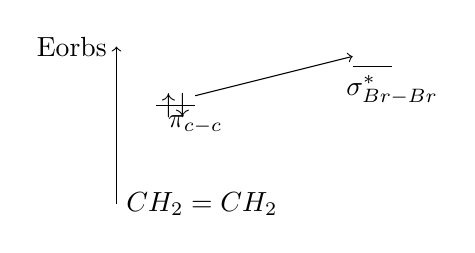
\begin{tikzpicture}[baseline=(current bounding box.center),scale=.5]
        \draw[->] (0,0)--(0,4)node[left]{Eorbs}node[right,pos=0]{$CH_2=CH_2$};
        \draw (1,2.5)--node{$\uparrow\downarrow$}+(1,0)node[below]{$\pi_{c-c}$};
        \draw[->] (2,2.75)--(6,3.75);
        \draw (6,3.5)--++(1,0)node[below]{$\sigma^*_{Br-Br}$};
    \end{tikzpicture}
    $\begin{matrix}
        \pi_{c-c}\text{上的一堆电子与}Br_2\text{的} \\
        \sigma^*_{Br-Br}\text{作用使反应发生}
    \end{matrix}$
\end{figure}

\begin{figure}[H]
    \centering
    \begin{tikzpicture}[scale=.5]
        \draw[->] (-5.5,-2)--(-5.5,4)node[right]{Eorbs};
        \draw (-3.6,-.75)--node{$\uparrow\downarrow$}+(1,0)node[left,pos=0]{2s};
        \draw (-4.6,2.25)--++(.5,0)node{$\uparrow$}-- ++(.5,0)node[left,pos=0]{$2p$}node[above]{C};
        \draw (-3.4,2.25)--++(.5,0)node{$\uparrow$}-- ++(.5,0);
        \draw[decorate,decoration={brace, amplitude=2}, line width=.8] (-2,3)--(-2,-2.5);
        \draw (-1.4,.25)--++(.5,0)node{$\uparrow$}-- ++(.5,0)node[below]{$2\times sp^2$};
        \draw (-.2,.25)--++(.5,0)node{$\uparrow$}-- ++(.5,0);
        \draw (1,.25)--++(.5,0)node{$\uparrow$}-- ++(.5,0)node[below]{$sp^2$};
        \draw[->] (1.5,-.75)--(3,-2.75);
        \draw[-,dashed] (2,.25)--(4,5);
        \draw[-,dashed] (2,.25)--(4,-1.5);
        \draw (1,2.75)--++(.5,0)node{$\uparrow$}-- ++(.5,0)node[left,pos=0]{$2p$};
        \draw[->] (1,2.25)--(-3.6,-2.75)node[below]{这个两个p轨道上各有一个$e^-$};
        \draw[-,dashed] (2,2.75)--(4,4);
        \draw[-,dashed] (2,2.75)--(4,1);
        \draw (4,-1.5)--node{$\uparrow\downarrow$}+(1,0)node[right]{$\sigma_{c-c}$};
        \draw (4,1)--node{$\uparrow\downarrow$}+(1,0)node[right]{$\pi_{c-c}$};
        \draw (4,4)--++(1,0)node[right]{$\pi^*_{c-c}$};
        \draw (4,5)--++(1,0)node[right]{$\sigma^*_{c-c}$};
        \draw (7,-.25)--++(.5,0)node{$\uparrow$}-- ++(.5,0)node[below,pos=.5]{$sp^2$};
        \draw[->] (7.5,-1.25)--(7,-2.75)node[below]{3个$sp^2\text{轨道各含有1个}e^-$,其中2个用来与H成键};
        \draw[-,dashed] (7,-.25)--(5,5);
        \draw[-,dashed] (7,-.25)--(5,-1.5);
        \draw (7,2.25)--++(.5,0)node{$\uparrow$}-- ++(.5,0)node[right]{$2p$};
        \draw[-,dashed] (7,2.25)--(5,4);
        \draw[-,dashed] (7,2.25)--(5,1);
        \draw (8.2,-.25)--++(.5,0)node{$\uparrow$}-- ++(.5,0)node[below]{$2\times sp^2$};
        \draw (9.4,-.25)--++(.5,0)node{$\uparrow$}-- ++(.5,0);
        \draw[decorate,decoration={brace, amplitude=2, mirror}, line width=.8] (11,2.5)--(11,-3);
        \draw (11.4,2.25)--++(.5,0)node{$\uparrow$}-- ++(.5,0);
        \draw (12.6,2.25)--++(.5,0)node{$\uparrow$}-- ++(.5,0)node[right]{2p};
        \draw (12.6,-.75)--node{$\uparrow\downarrow$}+(1,0)node[right]{2s};
    \end{tikzpicture}
\end{figure}

形成2个$\pi\text{轨道}
\begin{cases}
    \pi^*_{c-c} \\
    \pi_{c-c}
\end{cases}$
一个与相邻$sp^2\text{的C成键形成}
\begin{cases}
    \sigma^*_{c-c}(empty) \\
    \sigma_{c-c}(filled)
\end{cases}$

\textcolor{red}{\text{轨道重叠理论可以理解反应的发生}}

\subsection{总结}
\label{sec:2.2.3}
大多数反应依靠轨道重叠相互作用发生,而只有少数反应依靠电荷吸引

因此,用轨道重叠作用解释反应的发生具有代表性

\section{$Nu:^{\ominus}\& E^{\oplus}$}
\label{sec:2.3}
亲核试剂与亲电试剂

Nucleophile \& Electrophile

\subsection{回归两个反应}
\label{sec:2.3.1}
\begin{figure}[H]
    \centering
    \begin{tikzpicture}[scale=.5]
        \node[left] at (0,0) {\chemfig{\charge{45=\:,-45=\:}{O}(-[:135]H)(-[:-135]H)}};
        \draw[->,dashed] (.25,0)--(2.25,0);
        \node[right] at (2.25,0) {$\underset{HCHO}{\chemfig{(=[:0]O)(-[:135]H)(-[:-135]H)}}\delta^-$};
        \node[right] at (2.5,0) {$\delta^+$};
        \draw[->] (3.5,-.25)--(5.5,-.25);
        \draw[-] (3.7,-.1)--(3.7,-.4);
    \end{tikzpicture}
\end{figure}

\begin{figure}[H]
    \text{分子轨道理论观点}

    \centering
    \begin{tikzpicture}[scale=.5]
        \draw[->] (0,0)--(0,6)node[right]{Eorbs}node[right,pos=-.1]{$\qquad H_2O$}node[right,pos=.2]{O的$sp^3\text{轨道的1对}e^-$};
        \draw (1,2)--node{$\uparrow\downarrow$}+(1,0)node[right]{filled};
        \draw[->] (2,2.25)--(6,5.25)node[left,pos=.5]{overlap};
        \draw (6,5)--++(1,0)node[right]{empty};
        \node[right] at (6,4.5) {HCHO中空的$\pi^*_{c=o}$};
        \draw[->] (10,3)--(13,3)node[below,pos=.5]{形成新轨道};
        \draw (15,3)--++(1,0)node[below,pos=0]{$sp^3_o$};
        \draw[-,dashed] (16,3)--(16.5,1);
        \draw[-,dashed] (16,3)--(16.5,5);
        \draw (16.5,5)--++(1,0);
        \draw (16.5,1)--node{$\uparrow\downarrow$}+(1,0);
        \draw[-,dashed] (17.5,1)--(18,4);
        \draw[-,dashed] (17.5,5)--(18,4);     
        \draw (18,4)--++(1,0)node[right]{$\pi^*_{c=o}$};
    \end{tikzpicture}
    $\begin{matrix}
        \textcolor{red}{H_2O\text{中的O:给电子(donates electrons)}} \\
        \textcolor{red}{HCHO\text{中的C:收电子(accepts electrons)}}
    \end{matrix}$
\end{figure}

\begin{figure}[H]
    \qquad\qquad\qquad\qquad\qquad\qquad
    \begin{tikzpicture}[scale=.5]
        $\underset{C_2H_4}{\chemfig{(-[:-45]H)(=[:90] (-[:45]H)(-[:135]H))(-[:-135]H)}}$;
        \draw[->,dashed] (3,.5)--(5,.5)node[right]{Br-Br};
        \node[below] at (6,-1) {$Br_2$};
    \end{tikzpicture}
\end{figure}

\begin{figure}[H]
    \centering
    \begin{tikzpicture}[scale=.5]
        \draw[->] (0,1)--(0,6)node[right]{Eorbs}node[right,pos=0]{$C_2H_4\text{的filled}\pi_{c-c}$};
        \draw (1,2)--node{$\uparrow\downarrow$}+(1,0)node[right]{$\pi_{c-c}$};
        \draw[->] (2,2.25)--(6,5.25)node[left,pos=.5]{overlap};
        \draw (6,5)--++(1,0)node[right]{$\sigma^*_{Br-Br}$};
        \node[right] at (6,4.5) {$Br_2\text{的empty}\sigma^*_{Br-Br}$};
        \draw[->] (10,3)--(13,3)node[below,pos=.5]{形成新轨道};
        \draw (15,3)--node{$\uparrow\downarrow$}+(1,0)node[below,pos=0]{$\pi_{c-c}$};
        \draw[-,dashed] (16,3)--(16.5,1);
        \draw[-,dashed] (16,3)--(16.5,5);
        \draw (16.5,5)--++(1,0);
        \draw (16.5,1)--node{$\uparrow\downarrow$}+(1,0);
        \draw[-,dashed] (17.5,1)--(18,4);
        \draw[-,dashed] (17.5,5)--(18,4);     
        \draw (18,4)--++(1,0)node[right]{$\sigma^*_{Br-Br}$};
    \end{tikzpicture}
\end{figure}

\subsection{做出下列普适化定义}
\label{sec:2.3.2}
$^{\textcolor{red}{\star}}\text{反应中提供}e^-\text{作为亲核试剂}
\underset{\textcolor{red}{\text{一对}e^-}}{\underset{\textcolor{red}{\downarrow}}{(Nu:)}}
\text{反应中接受电子作为亲电试剂}\underset{\textcolor{red}{\text{形式正电荷}}}{\underset{\textcolor{red}{\downarrow}}{(E^{\oplus})}}$

$\newline$
用“弯曲箭头”表示电子(一对)流动

\begin{figure}[H]
    \begin{tikzpicture}[scale=.5]
        \draw[->,red] (0,0) arc (50:135:-1 and .6)node[black,left,pos=0]{反应通式\quad Nu:}node[black,right]{$E^{\oplus}\rightarrow Nu-E$};
    \end{tikzpicture}
\end{figure}

\subsection{用新的理论观点,讨论一个反应}
\label{sec:2.3.3}

\begin{figure}[H]
    \centering
    $\ce{NH_3 + BH_3 -> H_3N^{\oplus}-^{\ominus}BH_3}$

    \begin{tikzpicture}[scale=.5]
        \draw[draw=black] (-3.9,5.8)ellipse (.2 and .4);
        \filldraw[black] (-3.9,4.2)ellipse (.2 and .4);
        \node at (-4,5) {\chemfig{B(-[:180]H)(-[:30]H)(-[:-30]H)}};
        \draw[draw=black] (-4.85,4.15)ellipse (.2 and .4);
        \node at (-5,3) {\chemfig{\charge{90=\:}{N}(-[:-100]H)(-[:-60]H)(-[:-140]H)}};
        \draw[->] (0,0)--(0,5)node[right]{Eorbs}node[left,pos=.4]{\textcolor{red}{得$e^-\text{作}E^{\oplus}$}};
        \draw (1,4)--++(1,0)node[left,pos=0]{2p}node[above,pos=.5]{B};
        \draw[->,red] (1,3.75)--(-1,2.5);
        \draw[-,dashed] (2,4)--(4,5);
        \draw[-,dashed] (2,4)--(4,1);
        \draw (4,5)--++(1,0);
        \node[right] at (6,4.5) {N\quad \textcolor{red}{\text{失$e^-$作Nu}}};
        \draw (4,1)--node{$\uparrow\downarrow$}+(1,0);
        \draw[-,dashed] (6,2)--(5,5);
        \draw[-,dashed] (6,2)--(5,1);      
        \draw (6,2)--node{$\uparrow\downarrow$}+(1,0)node[right]{$sp^3$};
        \draw[-,dashed] (8,2)--(9,2);
        \draw[-,dashed] (5,1)--(9,1);
        \draw[->] (9,2)--(9,1);
        \draw[->,red] (9.25,1.1)--(9,0)node[below]{亲和位点为N的一对$sp^3$孤对电子};
    \end{tikzpicture}
\end{figure}

\begin{figure}[H]
    \qquad\text{若用弯曲箭头表示一对电子的流动}

    \qquad\text{则可以表示为}
    \quad
    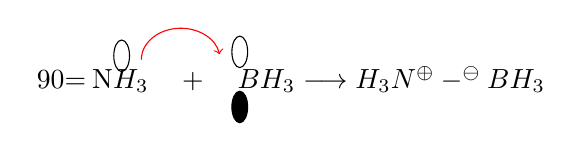
\begin{tikzpicture}[scale=.5]
        \draw[draw=black] (-3.3,.6)ellipse (.2 and .4);
        \draw[draw=black] (-.3,.7)ellipse (.2 and .4);
        \filldraw[black] (-.3,-.7)ellipse (.2 and .4);
        \draw[->,red] (-2.8,.5) arc (0:170:-1 and .8);
        \node at (1,0) {\chemfig{\charge{90=\:}{N}}$H_3\quad +\quad BH_3\longrightarrow H_3N^{\oplus}-^{\ominus}BH_3$};
    \end{tikzpicture}
\end{figure}

\begin{figure}[H]
    \begin{tikzpicture}[scale=.5]
        \draw[->] (0,0)--(0,5)node[right]{Eorbs};
        \draw (1,2.5)--++(1,0)node[above,pos=.5]{E};
        \draw[-,dashed] (2,2.5)--(3,4.5);
        \draw[-,dashed] (2,2.5)--(3,.5);
        \draw (3,4.5)--++(1,0);
        \draw (3,.5)--node{$\uparrow\downarrow$}+(1,0);
        \draw[-,dashed] (5,2)--(4,4.5);
        \draw[-,dashed] (5,2)--(4,.5);
        \draw (5,2)--node{$\uparrow\downarrow$}+(1,0)node[above]{Nu};
        \draw[-,dashed] (6,2)--(7,2);
        \draw[-,dashed] (4,.5)--(7,.5);
        \draw[->] (7,2)--(7,.5);
        \draw[->] (7.25,.6)--(6,-.5)node[left]{能量降};
        \draw (9,3.5)--++(1,0)node[above,pos=.5]{E};
        \draw[-,dashed] (10,3.5)--(11,5);
        \draw[-,dashed] (10,3.5)--(11,.5);
        \draw (11,5)--++(1,0);
        \draw (11,.5)--node{$\uparrow\downarrow$}+(1,0);
        \draw[-,dashed] (13,1.8)--(12,5);
        \draw[-,dashed] (13,1.8)--(12,.5);
        \draw (13,1.8)--node{$\uparrow\downarrow$}+(1,0)node[above]{Nu};
        \draw[-,dashed] (14,1.8)--(15,1.8);
        \draw[-,dashed] (12,.5)--(15,.5);
        \draw[->] (15,1.8)--(15,.5);
        \draw (17,4)--++(1,0)node[above,pos=.5]{E};
        \draw[-,dashed] (18,4)--(19,5.5);
        \draw[-,dashed] (18,4)--(19,.5);
        \draw (19,5.5)--++(1,0);
        \draw (19,.5)--node{$\uparrow\downarrow$}+(1,0);
        \draw[-,dashed] (21,1.3)--(20,5.5);
        \draw[-,dashed] (21,1.3)--(20,.5);
        \draw (21,1.3)--node{$\uparrow\downarrow$}+(1,0)node[above]{Nu};
        \draw[-,dashed] (22,1.3)--(23,1.3);
        \draw[-,dashed] (20,.5)--(23,.5);
        \draw[->] (23,1.3)--(23,.5);
        \draw[->] (6.5,-.7)--(23,-.7)node[above,pos=.4]{逐渐下降}node[below,pos=.35]{反应越难发生};
    \end{tikzpicture}
\end{figure}

亲核试剂与亲电试剂作用,两轨道重叠会有$\underset{\text{越打越有利于反应发生}}{\underset{\downarrow}{\text{“能量降”}}}$

\uwave{close in energy}\quad \textcolor{red}{\text{but能量降的大小取决于轨道间的接近程度,}}

\qquad\qquad\qquad\qquad \textcolor{red}{\text{越接近获得的能量降越大!}}

\begin{figure}[H]
    \begin{tikzpicture}[baseline=(current bounding box.center),scale=.5]
        \draw[->] (0,0)--(0,4)node[right]{Eorbs};
        \node[right] at (1,-.5) {$E_{sp^3_N}>E_{\sigma_{N-H}}$};
        \draw (1,1)--node{$\uparrow\downarrow$}+(1,0);
        \draw (2.2,1)--node{$\uparrow\downarrow$}+(1,0);
        \draw (3.4,1)--node{$\uparrow\downarrow$}+(1,0)node[right]{$\sigma_{N-H}$};
        \draw (2.2,2)--node{$\uparrow\downarrow$}+(1,0)node[right]{$sp^3_N$};
        \draw[->] (3.4,2.2)--(8,3.7);
        \draw (6.8,4.5)--++(1,0);
        \draw (8,4.5)--++(1,0);
        \draw (9.2,4.5)--++(1,0)node[right]{$\sigma^*_{B-H}$};
        \draw (8,3.5)--++(1,0)node[right]{$p_B$};
        \draw[<->] (9,3.5)--(9,2)node[right,pos=.5]{获得能量降最大};
        \draw[draw=black] (10.78,1.6)ellipse (.2 and .4);
        \draw[->] (11.2,1.5) arc (0:170:-1 and .4);
        \draw[draw=black] (13.8,1.7)ellipse (.2 and .4);
        \filldraw[black] (13.8,.3)ellipse (.2 and .4);
        \node at (14.8,1) {$\therefore\chemfig{\charge{90=\:}{N}}H_3\quad +\quad BH_3\longrightarrow H_3N^{\oplus}-^{\ominus}BH_3$};
        \node[right] at (13,4) {$E_{\sigma^*_{B-H}}>E_{p_B}$};
    \end{tikzpicture}

    \qquad\quad \text{N的$sp^3$与B的empty\quad p能量差最小}

    \text{以上就是前线轨道理论HOMO/LUMO的基础}
\end{figure}

\section{前线轨道理论简介}
\label{sec:2.4}
Review:\quad Nu:与$E^{\oplus}$能量越相近的轨道作用形成新轨道,新轨

\qquad\qquad\quad 道相对于原轨道的能量降越大

$\newline$
\begin{figure}[H]
    \qquad\qquad\qquad\qquad
    \begin{tikzpicture}[scale=.7]
        \text{一般的}\underline{\text{亲核试剂}}\text{与一般的}\underline{\text{亲电试剂}};
        \draw[->] (2.5,-.2)--(3,-.7)node[right]{\tiny 不止一条orb};
        \draw[->] (5,-.2)--(4.5,-.6);
    \end{tikzpicture}
\end{figure}

\begin{figure}[H]
    \begin{tikzpicture}[scale=.5]
        \draw[->] (0,5)--(0,6.2)node[right]{Eorbs};
        \draw (1,5)--++(1,0);
        \draw (1,4)--++(1,0);
        \draw (1,3)--++(1,0);
        \draw (1,2)--++(1,0);
        \draw[decorate,decoration={brace, amplitude=2}, line width=.8] (2.1,5)--(2.1,2);
        \draw[->] (2.2,3.5)--(3,5.2);
        \node[right] at (2.8,6.2) {同样考虑反应性$E^{\oplus}$的其它未占据轨道忽略};
        \draw (14,6.2)--++(1,0);
        \draw (14,5.5)--++(1,0);
        \draw (14,4.8)--++(1,0);
        \draw[decorate,decoration={brace, amplitude=2, mirror}, line width=.8] (13.9,6.2)--(13.9,4.8);
        \draw[->] (13.7,5.5)--(12.6,4)node[right]{Nu:提供电子,所以在反应中心的};
        \node[right] at (12.6,3.3) {空轨道可以忽略};
        \draw[very thick] (1,0)--++(1,0)node[above,pos=.5]{$E^{\oplus}$};
        \draw[->] (.8,0)--(.4,-1)node[left]{lowest};
        \node[right] at (-1.6,-1.5) {unoccupied};
        \node[right] at (-1.6,-2) {molecular};
        \node[right] at (-1.6,-2.5) {orbital};
        \node[right] at (-1.6,-3) {(LUMO)};
        \draw[-,dashed] (2,0)--(8,2.2);
        \draw[-,dashed] (2,0)--(8,-2);
        \draw[very thick] (8,2.2)--++(1,0);
        \draw[very thick] (8,-2)--node{$\uparrow\downarrow$}+(1,0);
        \draw[-,dashed] (14,-.5)--(9,2.2);
        \draw[-,dashed] (14,-.5)--(9,-2);
        \draw[very thick] (14,-.5)--node{$\uparrow\downarrow$}+(1,0)node[above,pos=.5]{Nu:};
        \draw[->] (15.2,-.5)--(16.2,-.5)node[right]{occupied};
        \node[right] at (16.2,0) {highest};
        \node[right] at (16.2,-1) {molecular};
        \node[right] at (16.2,-1.5) {orbital};
        \node[right] at (18.5,-.5) {(HOMO)};
        \draw (1,-3)--node{$\uparrow\downarrow$}+(1,0);
        \draw (1,-4)--node{$\uparrow\downarrow$}+(1,0);
        \draw (1,-5)--node{$\uparrow\downarrow$}+(1,0);
        \draw[decorate,decoration={brace, amplitude=2}, line width=.8] (2.1,-3)--(2.1,-5)node[right,pos=.5]{$E^{\oplus}$接收电子,所以它的占据轨道可以忽略}; 
        \draw (14,-2)--node{$\uparrow\downarrow$}+(1,0);
        \draw (14,-3)--node{$\uparrow\downarrow$}+(1,0);
        \draw (14,-4)--node{$\uparrow\downarrow$}+(1,0);
        \draw[decorate,decoration={brace, amplitude=2}, line width=.8] (15.1,-2)--(15.1,-4)node[right,pos=.5]{由于这些轨道没有}node[right,pos=.9]{最高电子占据轨道};
        \node[right] at (15.1,-4.5) {参加反应获得的};
        \node[right] at (15.1,-5.1) {能量降大所以忽略};
    \end{tikzpicture}
\end{figure}

\begin{figure}[H]
    \begin{tikzpicture}[scale=.5]
        \node[right] at (-.5,4.5) {所以\quad Nu:\& $E^{\oplus}$的本质};
        \draw[->] (0,0)--(0,4)node[right]{Eorbs}node[right,pos=.625]{HOMO}node[right,pos=.125]{好的Nu:有高能的HOMO};
        \draw (2.5,2.5)--node{$\uparrow\downarrow$}+(1,0);
        \draw (7,3)--++(1,0)node[right]{LUMO};
        \node[right] at (7,2.3) {好的$E^{\oplus}$有低能的LUMO};
    \end{tikzpicture}
    
    \qquad Nu:\qquad\qquad\qquad\qquad\quad $E^{\oplus}$

    \text{推论:以后我们只要谈Nu:\quad 只关注Nu:的HOMO}

    \qquad\qquad\qquad\qquad\quad \text{谈}$E^{\oplus}\quad \text{只关注}E^{\oplus}$\text{的LUMO}
\end{figure}

\subsection{哪些轨道常作Nu:的HOMO}
\label{sec:2.4.1}
\quad 哪些轨道/结构常作Nu:的HOMO

\quad 孤对电子所占据的轨道可作HOMO

\begin{figure}[H]
    \centering
    \begin{tikzpicture}[scale=.6]
        \node[left] at (1,.5) {含L.P.};
        \node at (2,0) {\chemfig{\charge{90=\:}{N}(-[:-90]H)(-[:-50]H)(-[:-130]H)}};
        \node at (4,0) {\chemfig{\charge{90=\:}{N}(-[:-90]R)(-[:-50]R)(-[:-130]R)}};
        \node at (6,0) {\chemfig{\charge{90=\:,-90=\:}{O}(-[:-30]H)(-[:-150]H)}};
        \node at (8.5,0) {\chemfig{\charge{90=\:,-90=\:}{O}(-[:-30]H)(-[:-150]R)}};
        \node at (2,-2) {\chemfig{\charge{90=\:}{P}(-[:-90]Me)(-[:-30]Me)(-[:-150]Me)}};
        \node at (5,-2) {\chemfig{\charge{90=\:,-90=\:}{S}(-[:-30]H)(-[:-150]Ph)}};
        \node at (7.5,-2) {\chemfig{\charge{90=\:,-90=\:}{S}(-[:-30]Me)(-[:-150]Me)}};
        \node at (14,0) {\chemfig{\charge{90=\:}{N}(-[:-90]H)(-[:-50]H)(-[:-130]H)}};
        \draw[draw=black] (14,1)ellipse (.2 and .4);
        \draw[->] (14.5,.5)--(15,.8)node[right]{$sp^3$};
    \end{tikzpicture}
\end{figure}

\begin{figure}[H]
    \centering
    \begin{tikzpicture}[scale=.6]
        \node[left] at (-1,10) {常见的阴离子也可以作Nu:};
        \node at (-5,8) {$\left [ \quad \chemfig{\charge{90=\:,-90=\:,0=\:}{O}(-[:180]H)}\quad \right ] ^{\ominus}\quad \left [ \quad \chemfig{\charge{90=\:,-90=\:,0=\:,180=\:}{Br}}\quad \right ] ^{\ominus}$};
        \node at (-5,6) {\chemfig{O(-[:-150]H)}\quad $\rightarrow sp^3$};
        \fill (-5.4,7) circle (1pt);
        \fill (-5.6,7) circle (1pt);
        \draw[draw=black] (-5.5,6.9)ellipse (.2 and .4);
        \fill (-5.4,5.4) circle (1pt);
        \fill (-5.6,5.4) circle (1pt);
        \draw[draw=black] (-5.5,5.5)ellipse (.2 and .4);
        \begin{scope}[rotate around={45:(-4.8,5.8)}]
            \draw[draw=black] (-4.8,5.8)ellipse (.2 and .4);
            \fill (-4.9,5.7) circle (1pt);
            \fill (-4.7,5.7) circle (1pt);
        \end{scope}
        \draw[->] (0,4)--(0,9)node[left]{Eorbs}node[right]{分析$^{\ominus}OH$的HOMO};
        \draw (1,7.5)--node{$\uparrow\downarrow$}+(1,0);
        \draw (2.2,7.5)--node{$\uparrow\downarrow$}+(1,0);
        \draw (3.4,7.5)--node{$\uparrow\downarrow$}+(1,0)node[right]{$sp^3_o$\quad 可作HOMO};
        \draw (2,6.5)--node{$\uparrow\downarrow$}+(1,0)node[right]{$\sigma_{O-H}$};
        \draw[draw=black] (-4.5,2.5)ellipse (.6 and .2);
        \node at (-4.5,2) {\chemfig{(-[:135]H)(=[:0] (-[:45]H)(-[:-45]H))(-[:-135]H)}};
        \shade[ball color=black!20] (-4.5,1.5)ellipse (.6 and .2);
        \draw[->] (0,0)--(0,4)node[left]{Eorbs};
        \node[left] at (-1,3.5){常见的$\pi$体系作Nu:};
        \draw (1,3)--node{$\uparrow\downarrow$}+(1,0)node[right]{$\pi_{c-c}$};
        \node[right] at (2,1.2) {$\sigma_{C-C},\sigma_{C-H}$};
        \node[left] at (-1.5,-.5){C-M物质作Nu:};
        \node at (-5,-2) {$\chemfig{B(-[:80]H)(<:[:-15]H)(<[:-75]H)(-[:-130]H)}$};
        \node at (-5.5,-1.8) {$\ominus$};
        \draw[<->] (-5.7,-5)--(-5.7,-3.5)node[right]{$\quad \delta^+$}node[right,pos=.3]{$\quad \delta^-$};
        \node at (-4,-5) {$\underset{\text{Li-C的E大.易断}}{\chemfig[atom sep=2.4em]{C(-[:90]Li)(<:[:-15]H)(<[:-75]H)(-[:-150]H)}}\equiv\quad ^{\ominus}CH_3$};
        \draw[->] (0,-6)--(0,-1)node[left]{Eorbs}node[right,pos=.8]{\qquad $C-M\quad \equiv\quad ^{\ominus}C+M^{\oplus}$}node[right,pos=.2]{\qquad $^{\ominus}BH_4\quad \equiv\quad BH_3+H^{\ominus}$};
    \end{tikzpicture}
\end{figure}

Nu:给出电子的过程可表示为

\begin{figure}[H]
    \centering
    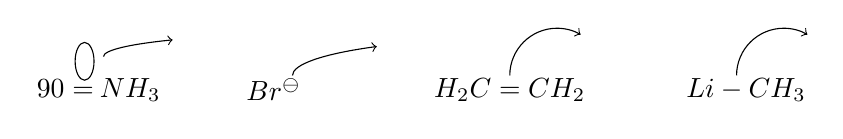
\begin{tikzpicture}[scale=.6]
        \draw[draw=black] (1,.9)ellipse (.2 and .4);
        \node at (1.3,.3) {$\chemfig{\charge{90=\:}{N}}H_3$};
        \draw[->] (1.4,1) arc (0:45:-5 and .5);
        \node at (5,.3) {$Br^{\ominus}$};
        \draw[->] (5.4,.6) arc (0:50:-5 and .8);
        \node at (10,.3) {$H_2C=CH_2$};
        \draw[->] (10,.6) arc (0:120:-1 and 1);
        \node at (15,.3) {$Li-CH_3$};
        \draw[->] (14.8,.6) arc (0:120:-1 and 1);
    \end{tikzpicture}
\end{figure}

\newpage
\subsection{哪些轨道作为HOMO/$E^{\oplus}$}
\label{sec:2.4.2}
哪些轨道$\&\text{结构作为HOMO}/E^{\oplus}$

$eg_1\text{有空轨道的结构可作}E^{\oplus}$,其中空轨道作LUMO

\begin{figure}[H]
    \qquad
    \begin{tikzpicture}[scale=.6]
        \node at (0,0) {$\overset{H^{\oplus}}{\chemfig{Al(-[:90]Cl)(<[:-60]Cl)(<:[:-120]Cl)}}$};
        \draw[draw=black] (0.8,-.3)ellipse (.4 and .2);
        \draw[draw=black] (-0.8,-.3)ellipse (.4 and .2);
        \node at (3,0) {$\overset{\text{1s轨道}}{\chemfig{B(-[:90]F)(<[:-60]F)(<:[:-120]F)}}$};
        \draw[draw=black] (3.7,-.3)ellipse (.4 and .2);
        \draw[draw=black] (2.3,-.3)ellipse (.4 and .2);
    \end{tikzpicture}
\end{figure}

$eg_2\underset{\bigtriangleup}{\uwave{\text{强}}}\uwave{\text{极性}}\pi\text{体系的}\pi^*$作为LUMO

$\chemfig{(=[:0]O)(-[:135])(-[:-135])}\quad \text{的}C\quad LUMO\quad \pi^*_{C-O}$

$\chemfig{(=[:0]NH)(-[:135])(-[:-135])}\quad \text{的}C\quad LUMO\quad \pi^*_{C-N}$

\begin{figure}[H]
    \qquad
    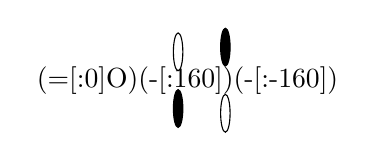
\begin{tikzpicture}[scale=.6]
        \draw[draw=black] (-.2,.6)ellipse (.1 and .4);
        \filldraw[black] (-.2,-.6)ellipse (.1 and .4);
        \node at (0,0) {\chemfig{(=[:0]O)(-[:160])(-[:-160])}};
        \filldraw[black] (.8,.7)ellipse (.1 and .4);
        \draw[draw=black] (.8,-.7)ellipse (.1 and .4);
    \end{tikzpicture}
\end{figure}

$eg_3\text{与电负性大的原子以}\sigma\text{键相连,}\sigma^*$可作为LUMO

HCl\quad 的$\sigma^*_{H-Cl}$

$H_3C-Br\quad \text{的}\sigma^*_{C-Br}$

Br-Br\quad 的$\sigma^*_{Br-Br}$

$E^{\oplus}$接受电子的过程可表示为

\begin{figure}[H]
    \qquad
    \begin{tikzpicture}[scale=.6]
        \node at (0,0) {$H^{\oplus}$};
        \draw[->] (-1.3,1) arc (80:170:-1 and .8);
        \node at (4,0) {\chemfig{B(-[:180]F)(-[:40]F)(-[:-40]F)}};
        \draw[draw=black] (4.1,.8)ellipse (.2 and .4);
        \filldraw[black] (4.1,-.8)ellipse (.2 and .4);
        \draw[->] (2.8,1.4) arc (70:135:-1 and .8);
        \node at (8,0) {\chemfig{(=[:0]O)(-[:135])(-[:-135])}};
        \draw[->] (6.5,0) arc (70:110:-1.2 and 3);
        \draw[->] (7.8,.2) arc (0:170:-.4 and .8);
        \node at (12,0) {H-Cl};
        \draw[->] (10.5,0) arc (70:110:-1.2 and 3);
        \draw[->] (12,.2) arc (0:170:-.2 and .8);
        \node[right] at (6.3,-2) {出现第2根箭头是第1根箭头作用后电子};
        \node[right] at (6.3,-3) {变多,需要把电子推出去};
    \end{tikzpicture}
\end{figure}

\section{画机理}
\label{sec:2.5}
\begin{figure}[H]
    \begin{tikzpicture}[scale=.7]
        \draw[decorate,decoration={brace, amplitude=2}, line width=.8] (0,0)--(0,2.5)
        node[left,pos=.5] {表现形式}node[right] {lewis结构式\quad 形式电荷=主族序数-未共享$e^-\text{数}-\frac{1}{2}$成键电子数}node[right,pos=0] {弯曲箭头};
        \draw[decorate,decoration={brace, amplitude=2}, line width=.8] (2.3,-1)--(2.3,1);
        \draw[->] (2.5,.8) arc (60:170:-.6 and .6);
        \draw[fishhook] (2.5,-.8) arc (60:170:-.6 and .6);
        \draw[->] (3.5,2.8) arc (0:90:-.6 and .6)node[right] {究竟是不是电荷maybe not};
        \draw[->] (-1,1) arc (0:140:-3.5 and -3)node[left,pos=.95] {展示}node[right,pos=.95] {何为机理\quad 展现有机反应历程的手段};
        \node[right] at (-2,-3.5) {$\underline{\text{思维过程}}$/理论基础:MOT/HOMO:LUMO};
        \draw[->] (0,-3)--(5.5,-1.5)node[below,pos=.9] {结合};
    \end{tikzpicture}
\end{figure}

\subsection{形式电荷的真实意义}
\label{sec:2.5.1}
\begin{figure}[H]
    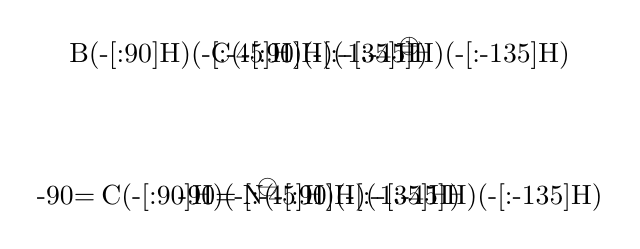
\begin{tikzpicture}[baseline=(current bounding box.center),scale=.6]
        \node at (0,0) {\chemfig{\charge{-90=\:}{C}(-[:90]H)(-[:-45]H)(-[:-135]H)}};
        \node at (.4,.2) {$\ominus$};
        \node at (3,0) {\chemfig{\charge{-90=\:}{N}(-[:90]H)(-[:-45]H)(-[:-135]H)}};
        \node at (0,3) {\chemfig{B(-[:90]H)(-[:-45]H)(-[:-135]H)}};
        \node at (3,3) {\chemfig{C(-[:90]H)(-[:-45]H)(-[:-135]H)}};
        \node at (3.4,3.2) {$\oplus$};
    \end{tikzpicture}
    \qquad
    $\begin{cases}
        BH_3\text{与}^{\oplus}CH_3 \\
        \\
        ^{\ominus}CH_3\text{与}NH_3
    \end{cases}$
\end{figure}

\begin{figure}[H]
    \begin{tikzpicture}[scale=.7]
        \node[right] at (0,2) {$\overset{C^{\ominus}}{\text{补足电荷}}\text{的记}\overset{N}{\text{号,不}}\text{是真正的电荷}$};
        \node[right] at (0,0) {\chemfig{C(=[:90]O)(-[:-30]H)(-[:-150]H)}\qquad \text{(真正有一点正电性)}};
        \node at (2,0) {$\delta\oplus$};
        \node at (2.3,1) {$\delta\ominus$};
        \node[right] at (10,2) {$\delta^+\overunderset{\delta^+}{\delta^+}{\chemfig{N(-[:0]Me)(-[:90]Me)(-[:-90]Me)(-[:180]Me)}}\delta^+$};
        \node at (12.3,2.3) {$\oplus$};
        \node[right] at (10,0) {形式电荷与部分电荷中心不重合};
    \end{tikzpicture}
\end{figure}

\begin{figure}[H]
    \begin{tikzpicture}[color=red,scale=.7]
        \node at (0,0) {$\underset{HNO_3}{\chemfig{N^{\oplus}(=[:0]O)(-[:130]^{\ominus}O)(-[:-130]HO)}}$};
        \node at (3,0) {$\underset{NO_3^-}{\chemfig{N^{\oplus}(=[:0]O)(-[:130]^{\ominus}O)(-[:-130]^{\ominus}O)}}$};
        \node at (6,0) {$\underset{-NO_2}{\chemfig{\charge{150=\.}{N_\oplus}(=[:0]O)(-[:-130]^{\ominus}O)}}$};
        \node at (9,0) {$\underset{HNO_2}{\chemfig{\charge{130=\:}{N}(=[:0]O)(-[:-130]HO)}}$};
        \begin{scope}[rotate around={45:(8.6,.95)}]
            \draw (8.6,.95)ellipse (.2 and .4);
        \end{scope}
        \node at (12,0) {$\underset{NO_2^-}{\chemfig{\charge{130=\:}{N}(=[:0]O)(-[:-130]^{\ominus}O)}}$};
        \begin{scope}[rotate around={45:(11.6,1)}]
            \draw (11.6,1)ellipse (.2 and .4);
        \end{scope}
        \node at (15,0) {$\underset{-NO_2}{\chemfig{\charge{130=\:,-130=\.}{N}(=[:0]O)}}$};
        \begin{scope}[rotate around={45:(14.2,.65)}]
            \draw (14.2,.65)ellipse (.2 and .4);
        \end{scope}
        \node at (1.5,-2.5) {$\overset{HPO_3\qquad \text{P含有3d}}{\chemfig{P(=[:0]O)(-[:130]OH)(=[:-130]O)}}$};
    \end{tikzpicture}
\end{figure}

\subsection{箭头表示什么}
\label{sec:2.5.2}
\begin{figure}[H]
    \begin{tikzpicture}
        \node[right] at (0,0) {最简单的例子:\quad $H_3O^{\oplus}\quad +\quad \overset{\ominus}{\chemfig{\charge{-90=\:}{O}}}H\longrightarrow 2H_2O$为例};
        \draw[->] (4,-.3) arc (0:180:.7 and -.4);
        \node[right] at (0,.5) {$eg_1\text{反应机理}\longrightarrow$第一根箭头};
        \node[right] at (0,1) {\quad 代表$\underset{overlap}{\text{轨道重叠}}\quad \uwave{HOMO\qquad LUMO}$};
        \draw[->] (3.3,1.3) arc (0:160:-.4 and .3);
        \draw[->] (3.8,.9)--(3.8,.5)node[right]{(};
        \node[right] at (0,1.5) {$\underset{\Downarrow}{\text{箭头表示什么}}$};
        \draw[fishhook] (2.5,2.5) arc (60:160:-.6 and .4)node[right]{一个$e^-$};
        \draw[->] (2.5,2) arc (60:160:-.6 and .4)node[right]{一对$e^-$};
    \end{tikzpicture}
\end{figure}

\begin{figure}[H]
    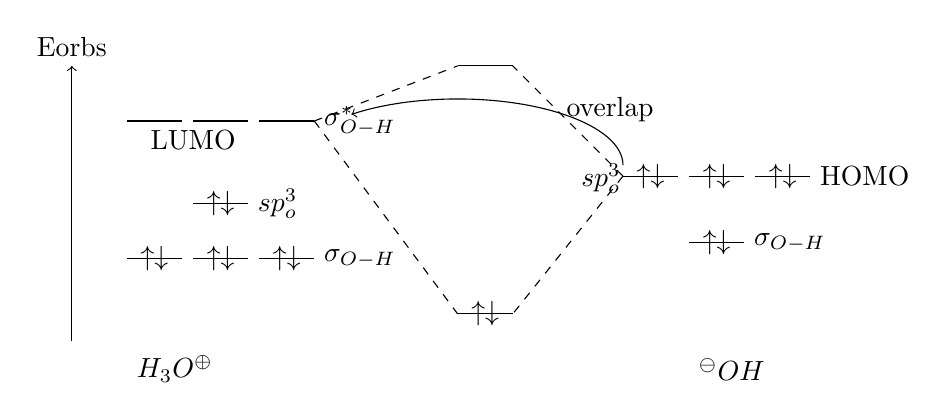
\begin{tikzpicture}[scale=.7]
        \draw[->] (0,0)--(0,5)node[above]{Eorbs}node[right,pos=-.1]{\qquad $H_3O^{\oplus}$};
        \draw (1,1.5)--node{$\uparrow\downarrow$}+(1,0);
        \draw (2.2,1.5)--node{$\uparrow\downarrow$}+(1,0);
        \draw (3.4,1.5)--node{$\uparrow\downarrow$}+(1,0)node[right]{$\sigma_{O-H}$};
        \draw (2.2,2.5)--node{$\uparrow\downarrow$}+(1,0)node[right]{$sp^3_o$};
        \draw (1,4)--++(1,0);
        \draw (2.2,4)--++(1,0)node[below,pos=0]{LUMO};
        \draw (3.4,4)--++(1,0)node[right]{$\sigma^*_{O-H}$};
        \draw[-,dashed] (4.4,4)--(7,5);
        \draw[-,dashed] (4.4,4)--(7,.5);
        \draw (7,5)--++(1,0);
        \draw (7,.5)--node{$\uparrow\downarrow$}++(1,0);
        \draw[-,dashed] (10,3)--(8,5)node[below,pos=.2]{$sp^3_o$}node[right,pos=.6]{overlap};
        \draw[-,dashed] (10,3)--(8,.5);
        \draw (10,3)--node{$\uparrow\downarrow$}+(1,0);
        \draw[->] (10,3.2) arc (0:130:3 and 1.2);
        \draw (11.2,3)--node{$\uparrow\downarrow$}+(1,0);
        \draw (12.4,3)--node{$\uparrow\downarrow$}+(1,0)node[right]{HOMO};
        \draw (11.2,1.8)--node{$\uparrow\downarrow$}+(1,0)node[right]{$\sigma_{O-H}$};
        \node[right] at (11.2,-.5) {$^{\ominus}OH$};
    \end{tikzpicture}
\end{figure}

\begin{figure}[H]
    \qquad\qquad\qquad
    \begin{tikzpicture}[baseline=(current bounding box.center)]
        \node at (0,0) {$\underset{LUMO:\sigma^*_{O-H}}{\chemfig{^{\oplus}O(-[:45]H)(-[:-50]H)(-[:-100]H)}}$};
        \draw[->] (3,.5) arc (0:160:1.5 and -.8)node[right,pos=0]{HOMO:$sp^3_o$};
        \node at (3.1,.8) {$\chemfig{\charge{-90=\:}{^{\ominus}O}}H$};
    \end{tikzpicture}

    \text{第一根箭头:找到HOMO$\&$LUMO并用一个箭头表示形成的新化学键}
\end{figure}

\begin{figure}[H]
    \text{通过第一根箭头作用后,会发现某些原子电子多了,就会有第二根箭头“推走”多的电子}

    eg:
    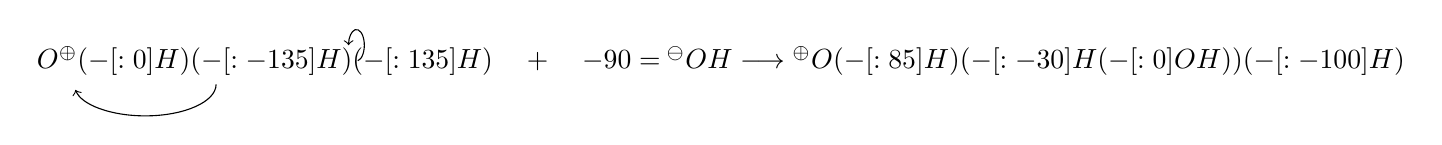
\begin{tikzpicture}[baseline=(current bounding box.center)]
        \node[right] at (0,0) {$\chemfig{O^{\oplus}(-[:0]H)(-[:-135]H)(-[:135]H)}\quad +\quad \chemfig{\charge{-90=\:}{^{\ominus}O}}H\longrightarrow\chemfig{^{\oplus}O(-[:85]H)(-[:-30]H(-[:0]OH))(-[:-100]H)}$};
        \draw[->] (2.4,-.3) arc (0:170:.9 and -.4);
        \draw[->] (4.2,0) arc (-80:180:.1 and .2);
    \end{tikzpicture}
\end{figure}

\subsection{推电子原则}
\label{sec:2.5.3}
推电子原则:
$\begin{cases}
    \text{为何推: 电子过多,装不下壳层} \\
    \text{推给谁: 邻近的能装下电子的原子} \\
    \text{推多少: 推成稳定结构} \\
    \text{谁被推: 能量最高的}e^-\text{对}/e^-\text{被推}
\end{cases}$

1.电子装不下壳层
$\begin{cases}
    \text{2周期}\quad 8e^- \\
    \text{3周期}\quad 18e^-
\end{cases}$

\begin{figure}[H]
    \qquad
    \text{2.3分子反应机理\quad $A+B+C\rightarrow D$\qquad 三分子发生有效碰撞概率极小}

    \qquad\qquad\qquad
    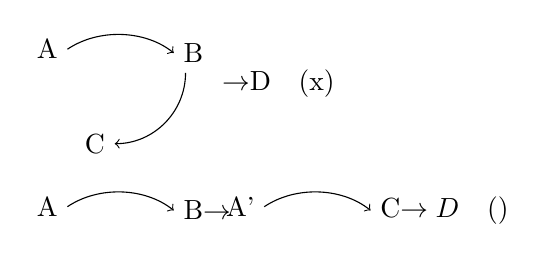
\begin{tikzpicture}
        \draw[->] (0,0) arc (50:135:-1 and .8)node[left,pos=0]{A}node[right]{B};
        \draw[->] (1.5,-.3) arc (0:90:.9 and -.9)node[left]{C}node[right,pos=.1]{\quad $\rightarrow$D\quad (x)};
        \draw[->] (0,-2) arc (50:135:-1 and .8)node[left,pos=0]{A}node[right]{B$\rightarrow$};
        \draw[->] (2.5,-2) arc (50:135:-1 and .8)node[left,pos=0]{A'}node[right]{C$\rightarrow D\quad (\checkmark)$};
    \end{tikzpicture}
\end{figure}

3.“箭头”贪多\quad 正确的(合理)的机理箭头$\le$3根

\qquad\qquad\qquad\qquad 机理每步反应都称“基元反应”

4.溶液相中不存在$H^{\oplus}\text{质子迁移用HA/}H_3O^{\oplus}$

